\graphicspath{ {./img/TheFEM/} }
\chapter{The Boundary Value Problem}

\section*{Preliminary}
In this section we review, in terms of governing equations and boundary conditions, the boundary value problem corresponding to the model of theory of elasticity. The first part of the chapter presents the stress and displacements formulation of the problem leading to the strong form. In the second part the problem is re-written in a weak sense leading to a form suitable for finite element algorithms. The chapter concludes with a third equivalent formulation, namely the principle of virtual work, which is obtained after minimization of the total potential energy functional. In a sense, this last statement of equilibrium is also a weak formulation useful for finite element implementation.

At the end of this chapter\footnote{{\bf This chapter, together with theoretical and computational learning activities is complemented by Jupyter Notebook 7.}} the student should be able to:


\begin{itemize}
\item[•] Understand the fundamental hypothesis leading to the model of linearized theory of elasticity.

\item[•] Understand the fundamental elements, including those of stress and strain, conforming the model of linearized theory of elasticity.

\item[•] Understand the problem of elasticity as a boundary value problem which can be equivalently formulated in differential and integral forms.

\item[•] Recognize valid solutions of the BVP specified over a particular domain and set of boundary conditions.

\end{itemize}

\section{Brief review of the linearized theory of elasticity model}
\subsection{Stress formulation}
Here we present a brief description of the boundary value problem governing the mechanical response of an elastic body. For a full discussion of the model and its mathematical aspects the reader is referred to \cite{shames1997elastic}. The equations are defined for a material point defined by its position $\vb{x}$ inside a body occupying a volume $V$ and bounded by the surface $S$ as shown in \cref{fig:blowL}. In a mathematical sense $V$ is the problem domain and the surface $S$ is the boundary where the solution is expected to be given in terms of prescribed (boundary) conditions (BCs).


\begin{figure}[H]
\centering
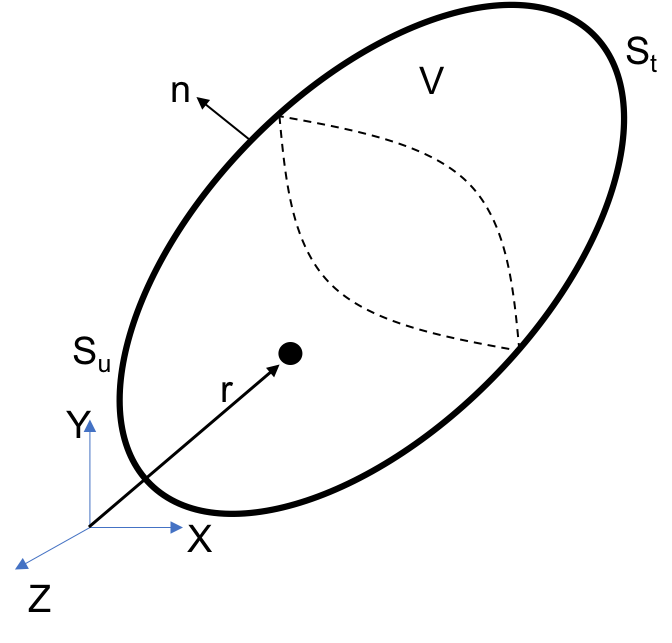
\includegraphics[width=7cm]{blow.png}
\caption{Problem domain.}
\label{fig:blowL}
\end{figure}

The governing equations (in terms of stresses) stem from application of the principle of conservation of linear momentum and conservation of moment of linear momentum to an arbitrary portion of the domain. Conservation of linear momentum leads to a set of 3 partial differential equations in the components of the stress tensor $\sigma_{ij}$ while conservation of moment of linear momentum leads to the symmetric character of this stress tensor. The resulting equations are given by:

\begin{equation} \label{eq:pde}
\begin{aligned}
&\sigma_{ij,j} + {f_i} = \rho\ddot{u}_i \quad \forall\ \vb{x} \in V,\, t \in \mathbb{R}^{+}\\
&\sigma_{ij}=\sigma _{ji}.
\end{aligned} 
\end{equation}

In \ref{eq:pde} $f_i$ is the vector of body forces and $u_i$ is the displacements vector where each dot represents a time differentiation. The set of governing equations in this stress formulation is complemented by boundary conditions specified in terms of the tractions vector $t_i^{\hat n}$ associated with a surface $S$ with normal direction $\hat{n}_{j}$. At any given surface this tractions vector is related to the stress tensor by:


\[
t_i^{\hat n} = \sigma_{ij} \hat{n}_{j} \quad \forall \in \vb{x} \in S.
\]



It must be noted that \cref{eq:pde} are a system of 6 equations in 12 unknowns (i.e., the 9 components of the stress tensor and the 3 components of the displacements vector) and therefore it is undetermined. To eliminate such indetermination we must relate the stresses to the changes in configuration. In the linearized model of elasticity the local changes in configuration are described in terms of changes of magnitude and internal distortions among material fibbers emanating from the material point. This kinematic information is described in terms of the strain tensor defined in terms of components of spatial gradients of the displacement vector as follows:


\begin{equation}\label{eq:kin}
\varepsilon_{ij} = \frac{1}{2}(u_{i,j} + u_{j,i}).
\end{equation}

Note that the term $\epsilon_{ij}$ is the symmetric component of the displacements gradient tensor. The components of the strain tensor describe the distortions and changes in magnitude (volumetric changes) of the material point in the continuum model. To complete the problem formulation the local changes in configuration must be related to the stress tensor at the material point through a constitutive law. The simplest stress-strain (constitutive) relationship is given by Hooke's law\footnote{Despite the name of \emph{law} used, this relation is not always valid, but is a good approximation for small strains.} as follows:

\begin{equation} \label{eq:Hooke}
\sigma_{ij} = 2\mu \varepsilon_{ij} + \lambda \varepsilon_{kk}\delta_{ij} \enspace .
\end{equation}

and where $\mu$ and $\lambda$ are material constants.

Note that \cref{eq:pde} to \cref{eq:Hooke} involves now a total of 18 equations in 18 unknowns and mathematically it is now a solvable system. However to find unique solutions the elastic solid must be subjected to properly specified boundary conditions.

\subsection{Displacement formulation}
The equilibrium equations in terms of stresses given by \cref{eq:pde} can be simplified after substituting \cref{eq:kin} in \cref{eq:Hooke} and the result in \cref{eq:pde} yielding after some manipulation:
\begin{equation} \label{eq:navier}
(\lambda  + \mu)u_{j,ij} + \mu u_{i,jj} + {f_i} = \rho \ddot{u}_i \quad \forall \vb{x} \in V,\, t \in \mathbb{R}^{+}.
\end{equation}

Note that now \cref{eq:navier} simultaneously satisfies equilibrium, kinematic relations and the constitutive law and they constitute a system of 3 partial second order differential equations in the 3 components of the displacement vector. For a unique solution these governing equations must be complemented with prescribed boundary values of the  displacement or its first order derivatives as given by:
 
\begin{equation}\label{eq:Wellbcs}
\begin{split}
&t_i^{\hat n} = \sigma _{ij} \hat n_{ij} \quad \forall\ \vb{x} \in S_t\\
& {u_i} = \bar{u}_i \quad \forall \vb x \in S_u
\end{split}
\end{equation}

and where ${S_t} \cup {S_u} = S$ and ${S_t} \cap {S_u} = \emptyset $. 

Notice that strictly speaking the problem involves time derivatives through the term $\rho \ddot{u}_i$ thus requiring also the specification of initial conditions in $t = 0$ for $u_i$ and $\dot{u}_i$. Here we will drop the inertial term and assume a static idealization and the problem becomes a boundary value problem (BVP) summarized next:


\begin{equation}
\begin{split}
&\left(\lambda  + \mu \right)u_{j,ij} + \mu u_{i,jj} + {f_i} = 0 \quad \forall \vb{x} \in V \\
&t_i^{\hat n} = \sigma _{ij} \hat n_{ij} \quad \forall\ \vb{x} \in S_t\\
& {u_i} = \bar{u}_i \quad \forall \vb x \in S_u
\end{split}
\label{eq:disps}
\end{equation}


In \ref{eq:disps} the boundary conditions specified by the traction vector $t_i^{\hat n}$


\[t_i^{\hat n} = \mu (u_{i,j} + u_{j,i}) \hat{n}_j + \lambda u_{k,k} \delta_{ij}\hat{n}_j \enspace ,\]

correspond to the natural boundary conditions. In fact these actually involve first order displacements derivative and as such they are Neumann boundary condition on $u_i$ while those specified in terms of the displacements vector $\bar u_i$ represent the essential boundary conditions.


\begin{tcolorbox}
The classical finite element algorithm to solve problems of elasticity interpolates nodal displacements and then computes derivatives to find strain and stress distributions as secondary variables, thus it is a displacement based solution analogous to Navier equations.
\end{tcolorbox}

%%%%%%
\paragraph*{Example: Two-dimensional idealization: Simple wedge under self-equilibrated loads}

The general equations governing the elasticity BVP can be represented by simplified two-dimensional versions under certain conditions satisfied by the geometry of the problem domain, the distribution of the external loads or specific values of some field components. In the most general cases these correspond to plane strain, plane stress and axy-symmetric problems. In the following example we present the special case of a two-dimensional idealization in a plane strain problem in which $\epsilon_{zz}=0$. 

Consider the double wedge of side $\ell$ and internal angle $2 \phi$ shown in \cref{fig:WEDGE}. It is assumed to be contained in the $X-Y$ plane, with loading conditions satisfying a plane strain idealization. The material is elastic and described by Lame constants $\lambda$ and $\mu$. The wedge is loaded by uniform tractions of intensity $S$ applied over its four faces in such a way that the wedge is self-equilibrated. We wish to find the elasticity solution for the stress, strain and displacement fields throughout the problem domain.
\begin{figure}[h]
\centering
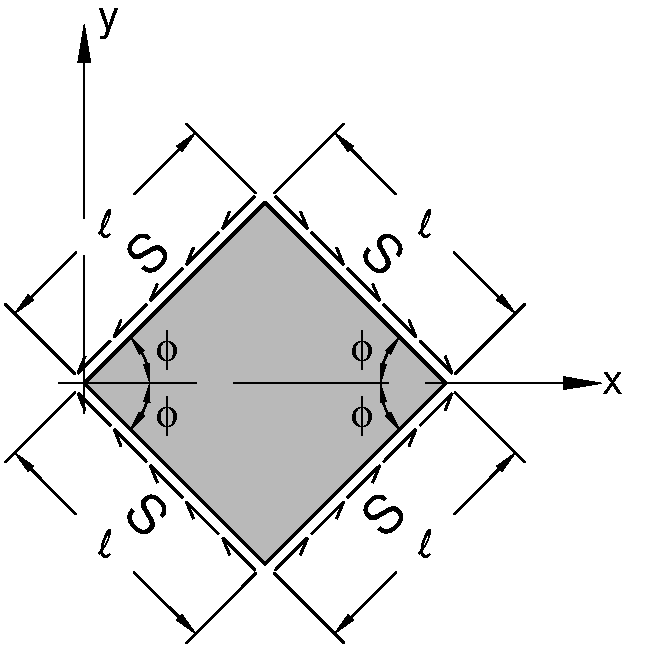
\includegraphics[width=9cm]{wedge.pdf}
\caption{2D Self-equilibrated wedge.}
\label{fig:WEDGE}
\end{figure}

%%%%

%\begin{figure}[H]
%\centering
%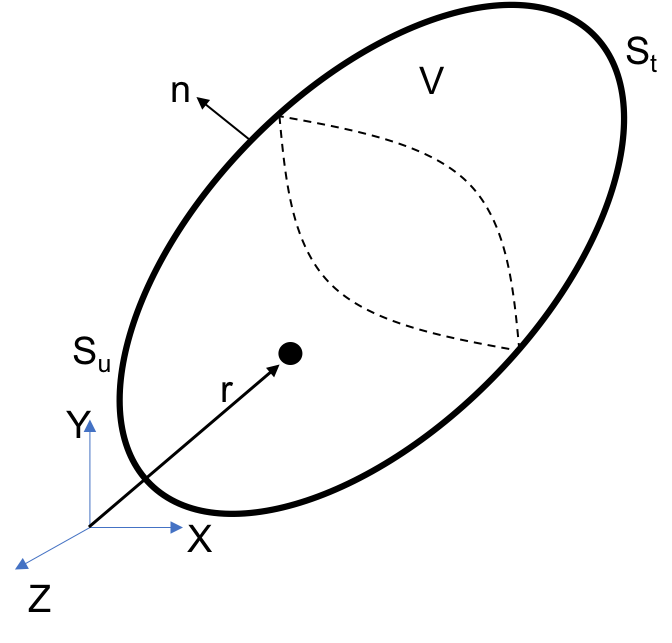
\includegraphics[width=7cm]{blow.png}
%\caption{Problem domain.}
%\label{fig:blow2}
%\end{figure}

%%%%


Under two-dimensional plane strain conditions the general three-dimensional stress equilibrium equations \ref{eq:pde} reduce to:
\begin{equation}
\begin{aligned}
&\pdv{\sigma_{xx}}{x} + \pdv{\tau_{xy}}{y}=0\\
&\pdv{\tau_{xy}}{x} + \pdv{\sigma_{yy}}{y}=0
\end{aligned}
\label{eq:equilibrium}
\end{equation}
while the kinematic relation \ref{eq:kin} reads
\begin{equation}
\begin{aligned}
\epsilon_{xx}& = \pdv{u}{x}\\
\epsilon_{yy}& = \pdv{v}{y}\\
\gamma_{xy}& = \pdv{u}{y} + \pdv{v}{x}
\end{aligned}
\label{eq:strain}
\end{equation}
where $u$ and $v$ are respectively the horizontal and vertical components of the displacement vector.

\subsubsection*{Stress field}

The stress field can be obtained by simple inspection from the traction boundary conditions prescribed over the inclined surfaces. Expressing the surface forces in terms of stresses gives:

\begin{align*}
\sum F_x &= 0 \longrightarrow - \ell S\cos(\phi)  + \sigma_{xx}\ell \sin(\phi) = 0\\
\sum F_y &= 0 \longrightarrow - \ell S\sin(\phi) - \sigma_{yy}\ell \cos(\phi)=0
\end{align*}

producing the following stress solution:

\begin{equation}
\begin{aligned}
\sigma_{xx}& = S \cot(\phi)\\
\sigma_{yy}& = -S\tan(\phi)\\
\tau_{xy}& = 0\, .
\end{aligned}
\label{eq:solution}
\end{equation}

In \cref{eq:solution} the condition $\tau_{xy}=0$ has been assumed  as suggested by the symmetries in the problem. Clearly the above stress field satisfies the local equilibrium equations, however for it to be the actual solution to the BVP it must also satisfy the boundary conditions.

\subsubsection*{Traction boundary conditions}
Let us verify that the above stress solution satisfies the traction BCs using the expression:

\[t_i^{\hat n} = \sigma_{ij} \hat n_{ij}.\]

Denoting the outward normals to the inclined surfaces of the wedge by $\hat{n}^1$,  $\hat{n}^2$, $\hat{n}^3$, $\hat{n}^4$ these are given by:
\begin{align*}
\hat{n}^1 &= -\sin(\phi)\hat{e}_{x}+\cos(\phi)\hat{e}_{y}\\
\hat{n}^2 &= -\sin(\phi)\hat{e}_{x}-\cos(\phi)\hat{e}_{y}\\
\hat{n}^3 &= +\sin(\phi)\hat{e}_{x}+\cos(\phi)\hat{e}_{y}\\
\hat{n}^4 &= +\sin(\phi)\hat{e}_{x}-\cos(\phi)\hat{e}_{y} \enspace ,
\end{align*}
where $\hat{e}_{x}$ and $\hat{e}_{y}$ are the reference unit vectors. Now, the components of the traction vector follow directly.

For the face with normal $\hat{n}^1$ we have

\begin{align*}
t_{x} &= -S\cos(\phi)\\
t_{y} &= -S\sin(\phi)
\end{align*}

similarly, over the face with normal $\hat{n}^2$ the traction reads
\begin{align*}
t_{x} &= -S\cos(\phi)\\
t_{y} &= +S\sin(\phi)
\end{align*}

over the face with normal $\hat{n}^3$

\begin{align*}
t_{x} &= +S\cos(\phi)\\
t_{y} &= -S\sin(\phi)
\end{align*}

and finally, over the face with normal $\hat{n}^4$;

\begin{align*}
t_{x} &= +S\cos(\phi)\\
t_{y} &= +S\sin(\phi) \enspace .
\end{align*}

Note that the above set of tractions found from the relation:

\[t_i^{\hat n} = \sigma_{ij} \hat n_{ij}\]

and after using the assumed stress field satisfies the problem boundary condition. Thus the stress field given by \cref{eq:solution} is the unique solution to the BVP for the self equilibrated wedge.

\subsubsection*{Strain field}
The strain field can be obtained after using the stress solution found in \cref{eq:solution} together with the constitutive law given by \cref{eq:Hooke} which for a plane strain idealization takes the form:
\begin{equation}
\begin{aligned}
\epsilon_{xx}& = \frac{1}{E}(\sigma_{xx} - \nu \sigma_{yy}) \\
\epsilon_{yy}& = \frac{1}{E}(\sigma_{yy} - \nu \sigma_{xx}) \\
\gamma_{xy}& = \frac{\tau _{xy}}{\mu}.
\end{aligned}
\label{eq:cons model}
\end{equation}

Particularizing we have:

\begin{equation}
\begin{aligned}
\epsilon_{xx}& = +\dfrac{S}{E}\left[\cot(\phi)+\nu \tan(\phi)\right] = +\dfrac{S}{E}K_{1}(\nu , \phi)\\
\epsilon_{yy}& = -\dfrac{S}{E}\left[\tan(\phi)+\nu \cot(\phi)\right] = -\dfrac{S}{E}K_{2}(\nu , \phi)\\
\gamma_{xy}& = 0.
\end{aligned}
\label{eq:strain part}
\end{equation}

\subsubsection*{Displacement field}
The displacement field is obtained after direct integration of the strains after using the fact that
\[\dd{u}_i = \epsilon_{ij} \dd{x}_j + \omega_{ij}\dd{x}_j\]
and the condition $\omega_{xy}=0$ (as a result of $\gamma_{xy} = 0$ which gives:

\begin{align*}
u &= +\dfrac{S}{E} K_{1}(\nu , \phi)x + A\\
v &= -\dfrac{S}{E} K_{2}(\nu , \phi)y + B
\end{align*}

and where $A$ and $B$ are integration constants while $K_{1}(\nu , \phi)$ and $K_{2}(\nu , \phi)$ are also constants that depend on Poisson's ratio and the wedge internal angle.

From the condition $u=0$ at $x=\ell\cos(\phi)$ we have that
\[A=-\dfrac{S}{E} K_{1}(\nu , \phi)\ell\cos(\phi)\]
then it follows that
\[u=\dfrac{S}{E} K_{1}(\nu , \phi)(x-\ell\cos(\phi)).\]

Similarly, from the condition $v=0$ at $y=0$ we have that $B=0$ from which
\[v=-\dfrac{S}{E} K_{2}(\nu , \phi)y\]

\begin{tcolorbox}
Notebook 7 in the REPO summarizes the BVP and uses interpolation to visualize the elastic field in the wedge solution.
\end{tcolorbox}


%%%%%
\section{Strong and weak forms of the BVP}
In this section we will present the elasticity BVP in an equivalent form suitable for finite element formulation. For that purpose, and just for completeness, we will repeat the differential formulation recently described and will immediately re-write it in an equivalent integral representation.
\subsection{Strong form}
The so-called strong form of the boundary value problem corresponds to the differential formulation just described, involving the governing equations and boundary conditions for a well posed problem. In the mathematical literature it is customary to denote the strong form as $\{ S \}$ and express it like:

Given $f_i$, $t_i^{\hat n}$ and ${\bar u_i}$ find ${u_i}:V \to \mathbb{R}$ such:

\begin{equation} \label{eq:navier_2}
\begin{split}
&(\lambda  + \mu)u_{j,ij} + \mu u_{i,jj} + f_i = 0 \quad \forall \vb{x} \in V \\
&t_i^{\hat n} = \sigma _{ij} \hat{n}_{ij} \quad \forall \vb{x} \in S_t\\
&u_i = \bar{u}_i \quad \forall \vb{x} \in S_u
\end{split}
\end{equation}


\subsection{Weak form}

\subsubsection*{A note on solution functions.}
\begin{itemize}
\item We are interested in developing methods to obtain approximate solutions to $\{S\}$.
\item The FEM is formulated starting from a statement equivalent to $\{ S \}$ in which we use trial functions until certain prescribed conditions are met.
\item We will look for solutions $u_i$ subject to the following conditions:
\begin{align*}
&u_i = \bar u_i \qquad \text{in} \qquad S_u\\
&\intL_S \left(\pdv{u_i}{x_j} \right)^2 \dd{S} < \infty
\end{align*}

\end{itemize}

The first condition corresponds to the satisfaction of the essential boundary condition, while the second corresponds to the functions being square integrable. The space of functions satisfying the above two conditions is denoted by $\varsigma$ and formally defined like
\[\varsigma = \left\{u_i\left| {u_i} \in H, {u_i} = \bar{u}_i \in S_u \right. \right\} \enspace .\]

On the other hand, in order to validate the introduced trial functions we also need testing functions $w_i$ also called in the FEM literature weighting or distribution functions. These functions are arbitrary apart from having to satisfy the following conditions:
\begin{align*}
&w_i = 0 \quad in \quad {S_u}\\
&\intL_S \left(\pdv{w_i}{x_j}\right)^2 \dd{S} < \infty
\end{align*}

In what follows we formally denote the space of these functions by $V$ and define it like
\[V = \left\{ w_i\left| w_i \in H, u_i = w_i=0 \in S_u \right. \right\} \enspace .\]

Here we will show that the equilibrium statement represented in the differential formulation can be described in alternative forms. In such description the continuity requirement for the trial functions is weaker than in the strong form leading to the term "weak" statement. Here this alternative representation will be denoted like $\{W\}$ and it reads;

Given $f_i$, $t_i^{\hat n}$ and ${\bar u_i}$ find ${u_i}:V \to \mathbb{R}$ and $\forall {w_i} \in V$ such:
\[\intL_V \sigma_{ij} w_{i,j}\, \dd{V} - \intL_V f_i w_i\, dV  - \intL_{S_t} t_i^{\hat n} w_i\, \dd{S} = 0\]

\subsubsection*{Proof 1:}
Let $u_i \in \varsigma $ be a solution to $\{S\}$ and let $w_i \in V $. Forming the inner product of the equilibrium statement given in \cref{eq:pde} with $w_i$ and forcing the integral over the domain to be zero we have
\[\intL_V (\sigma_{ij,j} + f_i ){w_i}\, dV = 0 \enspace ,\]
expanding the terms in the integrand and integrating by parts the first term on the left we have
\begin{align*}
&\intL_V \sigma _{ij,j} w_i\, \dd{V} + \intL_V f_i w_i\, \dd{V} = 0 \, ,\\
& -\intL_V w_{i,j} \sigma _{ij}\, \dd{V}  + \intL_S \sigma _{ij} \hat{n}_j w_i\, \dd{S}  + \intL\limits_V w_i f_i\, \dd{V} = 0\, ,
\end{align*}
since $w_i \in V$ it follows that $w_i = 0$ in $S_u$ from which
\begin{equation}\label{eq:weak}
\intL_V \sigma_{ij} w_{i,j}\, \dd{V} - \intL_V f_i w_i\, \dd{V}  - \intL_{S_t} t_i^{\hat n} w_i\, \dd{S} = 0\, .
\end{equation}

Now, considering that $u_i$ is solution of the strong form $\{S\}$ it must satisfy $u_i = \bar u_{i} \quad \in \quad S_u$ and as a result $u_i \in \varsigma$. On the other hand, since $u_i$ satisfies \cref{eq:weak} $\forall {w_i} \in V$ we have that $u_i$ satisfies the definition of weak solution specified in $\{ W \}$.

\subsubsection*{Proof 2:}
Let $u_i$ be a solution of $\{W\}$ and thus $u_i \in \varsigma$ which means that
\[u_i = \bar u_{i} \quad \in \quad S_u\]
and that it satisfies
\[\intL_V \sigma _{ij} w_{i,j}\, \dd{V} - \intL_V f_i w_i\, \dd{V} - \intL_{S_t} t_i^n w_i\, \dd{S} = 0 \enspace ,\]
integrating by parts,
\[-\intL_V \sigma_{ij,j} w_i \dd{V} + \intL_S \sigma_{ij} n_j w_i \dd{S}  - \intL_V f_i w_i \dd{V} - \intL_{S_t} {t_i^n} w_i \dd{S} = 0\]

Since $w_i \in V$ we have that $w_i=0$ in $S_u$ and therefore
\[\intL_V w_i(\sigma_{ij,j} + f_i) \dd{V} + \intL_{S_t} w_i( \sigma_{ij} n_j - t_i^n ) \dd{S} = 0 \]
from which

\begin{equation} 
\begin{split}
&\sigma_{ij,j} + f_i = 0 \quad \vb{x} \in V \\
&t_i^n = \sigma_{ij} n_j \quad \forall \vb{x} \in S_t\\
&{u_i} = \bar{u}_i \quad \forall \vb{x} \in S_u
\end{split}
\label{equil_2}
\end{equation}

which is once again the strong form of the problem given in \cref{eq:pde}.





\section{Variational formulation}
In this section we formulate the boundary value problem using the approach of the calculus of variations in which the governing PDEs and boundary conditions are obtained after finding the minimum (or maximum) of a functional according to a variational principle\footnote{According to Wikipedia \cite{wiki:variational_principle}

\begin{quotation}
A variational principle is a scientific principle used within the calculus of variations, which develops general methods for finding functions which minimize or maximize the value of quantities that depend upon those functions. For example, to answer this question: ``What is the shape of a chain suspended at both ends?" we can use the variational principle that the shape must minimize the gravitational potential energy.

According to Cornelius Lanczos, any physical law which can be expressed as a variational principle describes an expression which is self-adjoint. These expressions are also called Hermitian. Such an expression describes an invariant under a Hermitian transformation.
\end{quotation}}.

We will see that the weak form (and therefore also the strong form) can be obtained alternatively through the process of finding extreme values for a functional. We will illustrate this idea for the general case of theory of elasticity and then we will present particular examples.

\subsection*{Some vague definitions in the calculus of variations}
In variational calculus a {\bf functional} can be understood as a ``function" having as independent variables or arguments a space of vector functions and producing as a result (or dependent variable) a scalar. For instance, in the particular case of the theory of elasticity such a ``function" corresponds to the total potential energy functional $\Pi$ given by;
\begin{equation}\label{eq:Potential}
    \Pi(u_i) = \frac{1}{2}\int\limits_V \sigma_{ij}\varepsilon_{ij}\dd{V}  - \int\limits_V f_i\, u_i\dd{V}  - \int\limits_S t_i^{(n)} u_i\dd{S}
\end{equation}
and where the first term in the left hand side corresponds to the internal strain energy, while the last two terms are the work done by the external body and traction forces. The above functional has as independent variables the displacement vector and its spatial derivatives. This is indicated by the presence of the displacement vector $u_i$ in the expression $\Pi(u_i)$.

In variational calculus we are interested in finding a function $u_i$ that renders the functional $\Pi$ a maximum or a minimum. In loose terms, the analogous to the differential operator in calculus of functions is now termed the variational operator $\var$ (i.e., $\var$ is analogous to $\pdv{x_i}$). As such $\var{\Pi}$ acts over the function $u_i$ and its derivatives as follows
\[\var{\Pi}  = \pdv{\Pi}{u_i}\var{u_i} + \pdv{\Pi}{\left( \pdv{u_i}{x_j}\right)} \delta\left(\pdv{u_i}{x_j}\right) + \cdots + \pdv{\Pi}{\left( \pdv{^{n}u_i}{x_j \cdots \partial x_k}\right)} \delta\left( \pdv{^{n}u_i}{x_j \cdots \partial x_k}\right) \enspace .\]

The following rules apply to the variational operator $\delta$:
\begin{itemize}
\item For functionals $\Pi$ and $\Phi$ it follows that \[\var(\Pi  + \Phi) = \var{\Pi}  + \var{\Phi}\]
\item For functionals $\Pi$ and $\Phi$ it follows that \[\var(\Pi \Phi ) = \var{\Pi} \Phi  + \Pi \var{\Phi}\]
\item For a functional $\Pi$ and an integer $n$ it follows that \[\var(\Pi^n) = n(\Pi^{n - 1})\var{\Pi}\]
\item For a functional $\Pi$ it follows that \[\var{\int \Pi \dd{x}}  = \int \var{\Pi} \dd{x} \]
\end{itemize}

If the variational operator is applied to the functional $\Pi(u_i)$ it produces functions or variations in $u_i$ which are arbitrary and such $\var{u_i} \in V$ and $\var{u_i} = 0$ in $S_u$.

To find an extreme function in the calculus of variations we proceed like in differential calculus. Here we compute the first variation of the functional $\var{\Pi}$ and solve the variational equation
\begin{equation}\label{eq:vareq}
    \delta \Pi  = 0
\end{equation}
in the unknown function $u_i$. 

In the particular case of the total potential energy functional $\Pi$ this yields
\begin{equation}\label{eq:ClaPVW}
    \int\limits_V \sigma _{ij}\var{\varepsilon_{ij}}\dd{V}  - \int\limits_V f_i \var{u_i} \dd{V}  - \int\limits_{S_t} t_i^{(n)} \var{u_i}\dd{S}  = 0
\end{equation}
where we recognize the weak form of the BVP stated previously thus it is equivalent to the strong form:

\begin{equation} 
\begin{split}
&\sigma_{ij,j} + f_i = 0 \quad \vb{x} \in V \\
&t_i^n = \sigma_{ij} n_j \quad \forall \vb{x} \in S_t\\
&{u_i} = \bar{u}_i \quad \forall \vb{x} \in S_u
\end{split}
\label{equil_223}
\end{equation}

It becomes evident that the functions $\delta {u_i}$ in \cref{eq:ClaPVW} play the role of the test functions $w_i$ introduced in the weak form. On the other hand, since we have already shown that the weak and strong forms are equivalent we conclude that having the functional and the essential boundary conditions is equivalent to having the strong form of the problem. This result can be formalized in the following principle.


\subsection{Principle of minimum potential energy}
In the theory of elasticity the total potential energy $\Pi$ is the result of adding the elastic strain energy which is stored in the body upon deformation and the potential energy (work) imparted to the body by the applied forces. The principle of virtual work states that the body is in equilibrium when this total potential energy reaches a minimum. This is equivalent to stating that an equilibrium configuration is attained when an infinitesimal variation from the position of minimum potential energy involves null changes in energy. This implies the variational condition:
\begin{equation}\label{vareq2}
    \delta \Pi  = 0.
\end{equation}

The above principle leads to the so-called principle of virtual displacements stated as follows\footnote{See Bathe pp 156.}:

{\bf ``The equilibrium of the body requires that for any compatible small virtual displacements satisfying the condition of being zero at $S_u$, imposed on the body in its state of equilibrium, the total internal virtual work is equal to the total external virtual work"
\[\int\limits_V \sigma _{ij}\var{\varepsilon_{ij}}\dd{V}  - \int\limits_V f_i\delta u_i\dd{V}  - \int\limits_{S_t} t_i^{(n)}\var{u_i}\dd{S}  = 0\]
where $\var{u_i}$ are the virtual displacements and $\var{ \varepsilon_{ij}}$ are the corresponding virtual strains. }

Comparing the virtual work principle with the weak formulation given in \cref{eq:weak} we identify $\var{u_i}$ with the test functions $w_i$. As such the PVW takes the form of a powerful tool to test if a body is in equilibrium for a given solution (represented by the trial functions). In what follows we illustrate the use of the principle through some examples corresponding to problems in Bathe's textbook.

\subsubsection*{Problem\footnote{3.15 from Finite Element Procedures}}
Establish the differential equation of equilibrium of the problem shown and the boundary conditions. Determine whether the differential operator of the problem is symmetric and positive definite and prove your answer.\cite{book:bathe}
\begin{figure}[H]
    \centering
    \includegraphics[width=10cm]{{Bathe3.15}.pdf}
    \caption{Rod with varying cross-sectional area. The Young's modulus is E.}
    \label{fig:bathe3.15}
\end{figure}


\begin{align*}
\Pi &= \frac{1}{2}\int\limits_0^L \sigma_{xx}\varepsilon_{xx}A(x)\dd{x} + \frac{1}{2}ku_0^2 - R u_L \\
 &= \frac{1}{2}\int\limits_0^L EA(x)\left( \dv{u}{x}\right)^2 \dd{x} + \frac{1}{2}ku_0^2  - R u_L \enspace.
\end{align*}

The first variation for this functional is
\[\var{\Pi}  = \int\limits_0^L EA(x)\dv{u}{x}\dv{\var{u}}{x}\dd{x} + k u_0\var{u_0}  - R\var{u_L} \enspace .\]

If we integrate by parts, we obtain
\[\var{\Pi}  =  - \int\limits_0^L \dv{x}\left[EA(x)\dv{u}{x}\right]\var{u}\dd{x} + \left. EA(x)\dv{u}{x}\var{u} \right|_0^L + k{u_0}\var{u_0}  - R\var{u_L}\]
from which
\begin{align*}
&\dv{x}\left[EA(x)\dv{u}{x}\right] = 0\\
&\left. EA(x)\dv{u}{x}\right|_{x=0} = k u_0\\
&\left. EA(x)\dv{u}{x}\right|_{x=L} = R
\end{align*}


\begin{tcolorbox}
The statements:

\[\int\limits_V \sigma _{ij}\var{\varepsilon_{ij}}\dd{V}  - \int\limits_V f_i \var{u_i} \dd{V}  - \int\limits_{S_t} t_i^{(n)} \var{u_i}\dd{S}  = 0\]

complemented by the condition $u_i={\overline u}_i \quad \forall \vb{x} \in S_u$

and

\begin{align*} 
\begin{split}
&\sigma_{ij,j} + f_i = 0 \quad \vb{x} \in V \\
&t_i^n = \sigma_{ij} n_j \quad \forall \vb{x} \in S_t\\
&{u_i} = \bar{u}_i \quad \forall \vb{x} \in S_u
\end{split}
\end{align*}

are equivalent.

\end{tcolorbox}





\paragraph*{The Hu-Washizu Variational Principle-Alternative formulation of the variational statement\footnote{4.35 from Finite Element Procedures}}

Consider the Hu-Washizu functional:
\begin{equation}
\Pi^* = \Pi  - \intL_V \lambda_{ij}^\varepsilon (\varepsilon_{ij} - L_{ijk} u_k)\dd{V}  - \intL_{S_u} \lambda_i^u(u_i^{S_u} - \bar{ u}_i)\dd{S}
\label{eq:Hu}
\end{equation}
where
\begin{itemize}
\item $\Pi$: is the potential energy functional.
\item $L_{ijk}$ is a differential operator such $\varepsilon_{ij} = L_{ijk} u_k$.
\item $S_u$ surface where essential boundary conditions are prescribed.
\item $\lambda_{ij}^\varepsilon $ and $\lambda_i^u$ are Lagrange multipliers.
\end{itemize}

Using the condition $\var{\Pi^*} = 0$ derive for the interior of the body the equilibrium equations
\[\sigma_{ij,j} + f_i = 0\]
the strain-displacement relationship
\[\varepsilon_{ij} = L_{ijk} u_k\]
and the constitutive equation
\[\sigma_{ij} = C_{ijkl} \varepsilon_{kl}\]
and at the surface of the body the relation between the stress tensor and the applied tractions vector at $S_t$
\[t_i = \sigma_{ij} n_j\]
the relation between the stress tensor and the unknown tractions vector (or reactions) at $S_u$
\[t_i = \tilde{\sigma_{ij}} n_j\]
and the essential boundary condition at $S_u$
\[u_i = \tilde{u}_i\]
We want to determine the Euler equations resulting from the condition $\var{\Pi}^* = 0$. Applying the variational operator we have
\begin{equation}
\begin{aligned}
\var{\Pi}^*& = \var{\Pi}  - \intL_V \var{\lambda}_{ij}^{\varepsilon}  (\varepsilon_{ij} - L_{ijk} u_k)\dd{V}- \intL_V \lambda_{ij}^\varepsilon (\var{\varepsilon}_{ij} - L_{ijk}\var{u}_k)\dd{V} \\
&-\intL_V \var{\lambda}_i^u (u_i^{S_u} - \bar u_i)\dd{S} - \intL_V \lambda _i^u \var{u}_i^{S_u} \dd{S}
\end{aligned}
\end{equation}
and
\begin{equation}
\begin{aligned}
\var{\Pi}^* =& \intL_V C_{ijkl} \varepsilon_{kl} \var{ \varepsilon}_{ij}\dd{V} - \intL_{S_t} t_i \var{u_i} \dd{S}  - \intL_V f_i \var{u_i}\dd{V}\\
  &- \intL_V \lambda_{ij}^{\varepsilon} \var{\varepsilon}_{ij}\dd{V}  + \intL_V \lambda_{ij}^{\varepsilon} L_{ijk}\var{u_k}\dd{V} - \intL_V \delta \lambda_{ij}^\varepsilon (\varepsilon_{ij}\\
  &- L_{ijk} u_k)\dd{V} - \intL_S \var{\lambda}_i^u (u_i^{S_u} - \bar {u}_i)\dd{S} - \intL_{S_u} \lambda _i^u\var{u_i}\dd{S} = 0
\end{aligned}
\end{equation}
using
\[\intL_V (\lambda_{ij}^\varepsilon \var{u_i}){,_j}\dd{V} =  \intL_V \lambda_{ij}^\varepsilon \var{u}_{i,j}\dd{V}  + \intL_V \lambda_{ij,j}^\varepsilon \var{u_i}\dd{V} \]

In the above we can write
\begin{align*}
\intL_V \lambda_{ij}^\varepsilon L_{ijk}\var{u_k}\dd{V} & = \intL_V (\lambda_{ij}^\varepsilon \var{u_i})_{,j}\dd{V} - \intL_V \lambda_{ij,j}^\varepsilon \delta {u_i}\dd{V}\\
& = \intL_{S_t} \lambda_{ij}^\varepsilon \var{u_i}\hat {n}_j\dd{S}  - \intL_V \lambda_{ij,j}^\varepsilon \var{u_i}\dd{V}
\end{align*}
therefore
\begin{align*}
\delta \Pi^* =& \intL_V (C_{ijkl}\varepsilon_{kl} - \lambda_{ij}^\varepsilon) \var{\varepsilon}_{ij}\dd{V} - \intL_{S_t} t_i \var{u}_i\dd{S} - \intL_V f_i \var{u}_i\dd{V}\\
  &+ \intL_{S_t} \lambda_{ij}^\varepsilon \var{u_i}\hat{n}_j\dd{S}  - \intL_V \lambda_{ij,j}^\varepsilon \delta {u_i}\dd{V} - \intL_V \delta \lambda _{ij}^\varepsilon (\varepsilon_{ij}\\
  &- L_{ijk} u_k)\dd{V}  - \intL_{S_u} \var{\lambda}_i^u (u_i^{S_u} - \bar{u}_i)\dd{S} - \intL_{S_u} \lambda_i^u \var{u_i} \dd{S}  = 0\\
=& \intL_V (C_{ijkl}\varepsilon_{kl} - \lambda_{ij}^\varepsilon) \var{\varepsilon}_{ij}\dd{V}
+ \intL_{S_t} (\lambda_{ij}^\varepsilon \hat{n}_j - t_i)\delta {u_i}\dd{S}\\
  &- \intL_V (\lambda_{ij,j}^\varepsilon  + f_i) \var{u_i}\dd{V}
- \intL_V (\varepsilon_{ij}- L_{ijk} u_k) \var{\lambda} _{ij}^\varepsilon\dd{V}\\
  &- \intL_{S_u} (u_i^{S_u} - \bar{u}_i) \var{\lambda}_i^u\dd{S}  - \cancel{\intL_{S_u} \lambda _i^u \var{u}_i^{S_u}\dd{S}} = 0
\end{align*}

Now, imposing the conditions $\var{\varepsilon}_{ij} \neq 0$, $\var{\lambda}_{ij}^\varepsilon  \neq 0$, $var{u}_i \neq 0$ in $S_t$, $\var{u}_i \neq 0$ in $V$ and $\var{\lambda}_i^u \neq 0$ in $S_u$ we have
\begin{align}
&\lambda_{ij}^\varepsilon  = C_{ijkl} \varepsilon_{kl}\\
&\varepsilon_{ij} = L_{ijk} u_k\\
t_i &= \lambda_{ij}^\varepsilon \hat{n}_j\\
&\lambda_{ij,j}^\varepsilon  + {f_i} = 0\\
&u_i^{S_u} = \bar{u}_i \enspace .
\end{align}


%%%%%





\paragraph*{Proposed problems}

\begin{enumerate}

\item \label{punto01} For the following displacements field:
\[\mathbf{u} = a(x^2 - 5y^2)\hat{\mathbf{i}} + (2ax y)\hat{\mathbf{j}} \]

\begin{enumerate}
\item Find the strain tensor.
\item Find the principal strains.
\item Find the principal stresses.
\end{enumerate}


\item \label{punto02} \Cref{fig:vigaV} shows a cantilever beam of unitary cross section with a distributed load applied at the free edge and following a parabolic distribution given by:

\[\mathbf{t} = \frac{Pc^2}{2I}\left(1-\frac{y^2}{c^2}\right)\hat{\mathbf{j}}\].

The stress solution is given by:
\begin{align*}
&\sigma_{xx} = -\frac{P}{I}xy \enspace ,\\
&\sigma_{yy} = 0 \enspace ,\\
&\sigma_{xy} = -\frac{P}{2I}(c^2 - y^2) \enspace .
\end{align*}

while the displacement field reads:

\begin{align*}
&u_{x} = \left(\frac{1}{G} - \frac{\nu}{E}\right)\frac{Py^3}{6I} + \left(\frac{l^2}{E} - \frac{x^2}{E} - \frac{c^2}{G} \right)\frac{Py}{2I} \enspace ,\\
&u_{y} = \frac{\nu P xy^2}{2EI} + \frac{Px^3}{6EI} - \frac{Pl^2x}{2EI} + \frac{Pl^3}{3EI} \enspace ,
\end{align*}
where $G=E/(2 + 2\nu)$ is the shear modulus and $I$ is the moment of inertia of the cross section.

\begin{figure}[H]
	\centering
	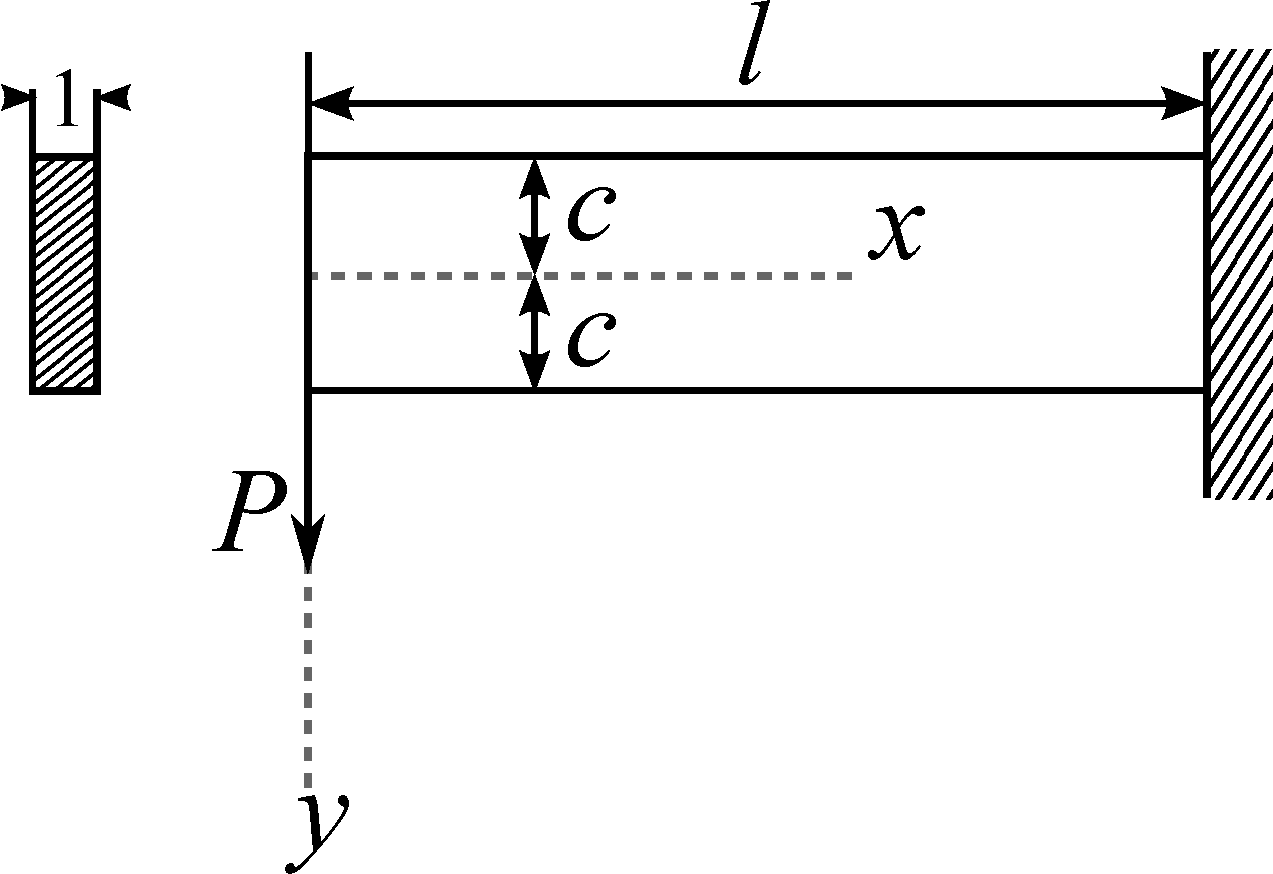
\includegraphics[height=5cm]{Viga_Voladizo.pdf}
	\caption{Cantilever beam with a distributed load at the end.}
	\label{fig:vigaV}
\end{figure}


%\begin{figure}[H]
%\centering
%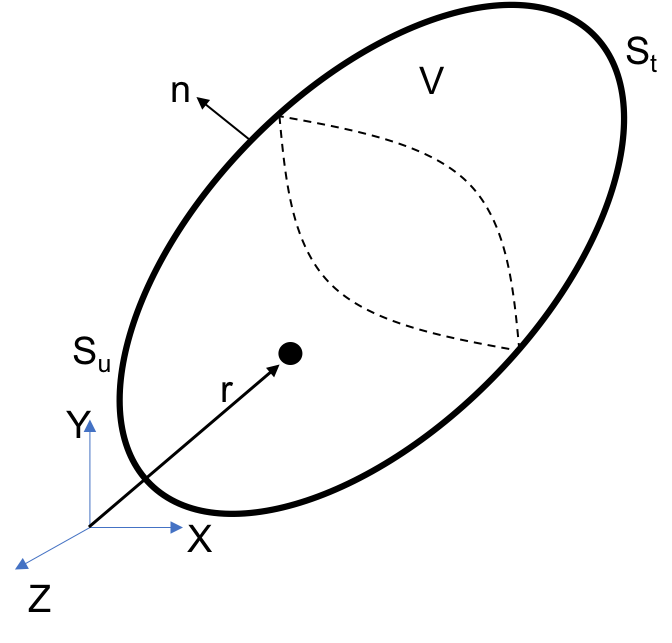
\includegraphics[width=7cm]{blow.png}
%\caption{Problem domain.}
%\label{fig:blow}
%\end{figure}

\begin{enumerate}
\item Identify the displacement and traction boundary conditions of the problem.
\item Verify that the stress and displacement solutions satisfy the proper boundary conditions.
\item  Find the region of the beam under tension and compression and thus its neutral axis. Find the equation corresponding to the displacement of the neutral axis and compare it with beam theory.
\end{enumerate}

\end{enumerate}



